% credits: http://tex.stackexchange.com/a/193404
\def\n{7}
\def\nminusone{6}
\footnotesize{
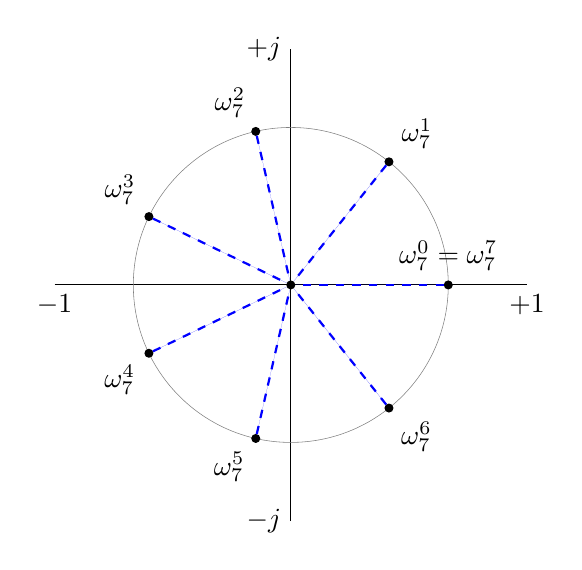
\begin{tikzpicture}[
  dot/.style={draw,fill,circle,inner sep=1pt}
  ]
  \draw[-] (-3,0) -- (3,0) node[below] {$+1$};
  \node[below] at (-3,0) {$-1$};
  \draw[-] (0,-3) -- (0,3) node[left] {$+j$};
  \node[left] at (0,-3) {$-j$};
  \draw[help lines] (0,0) circle (2);

  \node[dot] (zero) at (0,0) {};
  % default line width=0.4pt
  \foreach \i in {1,...,\nminusone} {
    \node[dot,label={\i*360/\n-(\i==\n)*45:$\omega_{\n}^{\i}$}] (w\i) at (\i*360/\n:2) {};
    %\draw[->,dashed] (O) -- (w\i);
    \path[draw=blue,fill=blue,dashed,line width=0.8pt] (w\i) -- (zero);
  }
  % draw 0 and n
  \node[dot,label={90:$\omega_{\n}^{0} = \omega_{\n}^{\n}$}] (w0) at (0:2) {};
  %\draw[->,dashed] (zero) -- (w0);
  \path[draw=blue,fill=blue,dashed,line width=0.8pt] (w0) -- (zero);
\end{tikzpicture}
}
